\section{Approach}
\label{sec:alignmentAlg}
%(mostly along the lines of my presentation for the USCMS workshop because it was time when I was the most active)

%Why align?\\
%How to align?\\
%When align?\\
%How to check that your alignment is good?\\



The concept of the track-based alignment can be illustrated in the example of the alignment of a toy tracker. When a charged particle passing through a detector (Fig.~\ref{fig:toyTracker_part1}, top left) it crosses a toy tracker which consists of six flat equidistant modules (Fig.~\ref{fig:toyTracker_part1}, top right). If the modules were placed exactly at their designed positions, we would observe the hits exactly at the points where the track crosses modules at the points of ideal geometry (Fig.~\ref{fig:toyTracker_part1}, middle left). However, in a reality the positions and tilts of the modules are different from ones suggested by the ideal geometry (Fig.~\ref{fig:toyTracker_part1}, middle right). Hits, indeed, are recorded at the places where modules are actually mounted, not at the design ideal places (Fig.~\ref{fig:toyTracker_part1}, bottom left). If we assumed a tracker to be ideal and a track to be smooth, we would see that our hits are off-track (Fig.~\ref{fig:toyTracker_part1}, bottom right). So, we recalculate positions of the modules so that all the hits are laying on the same smooth track (Fig.~\ref{fig:toyTracker_part2}, top left). But these recalculated positions still do not coincide with the actual positions (Fig.~\ref{fig:toyTracker_part2}, top right). Then we record more and more tracks (Fig.~\ref{fig:toyTracker_part2}, middle left and right). We take into account them all and determine the alignment parameters with necessary precision (Fig.~\ref{fig:toyTracker_part2}, bottom left and right) minimizing residuals between measured and predicted hits.

\begin{figure}[htb]
    \begin{center}
          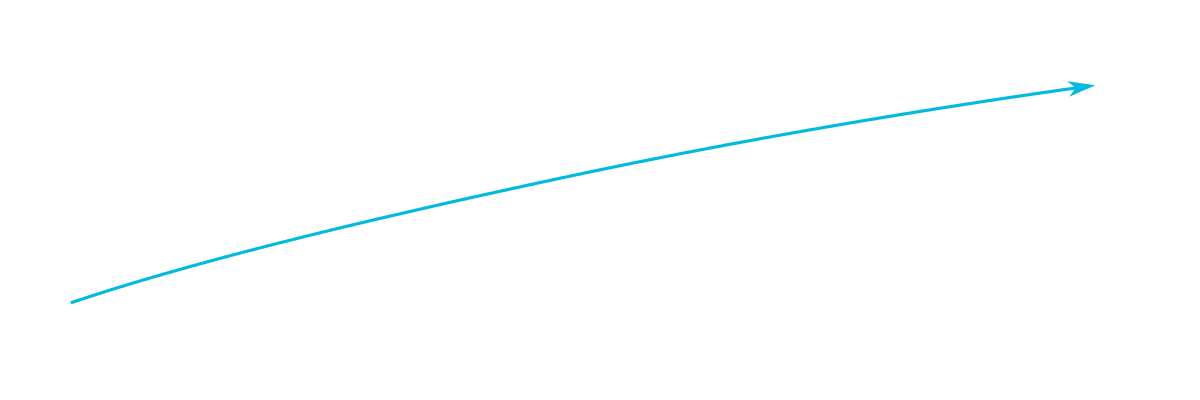
\includegraphics[width=0.45\textwidth]{../figs/Alignment/toyTracker01.png}
          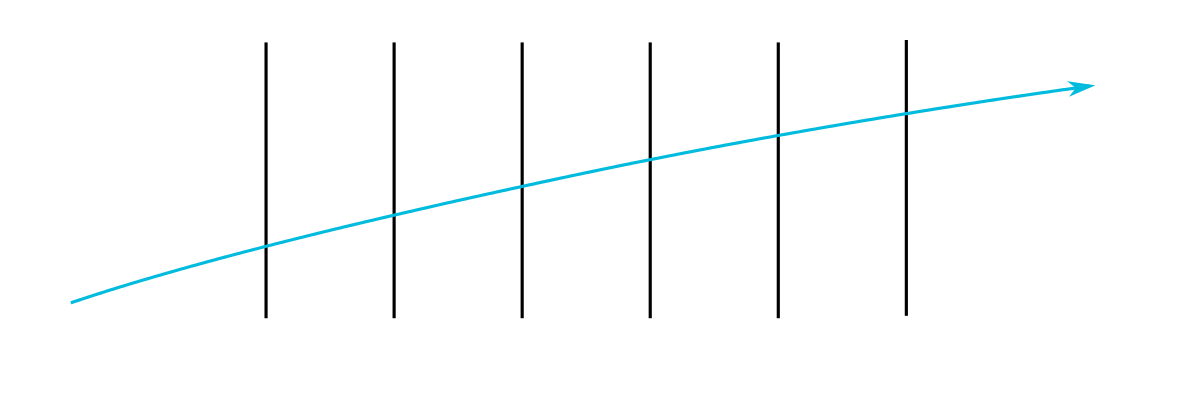
\includegraphics[width=0.45\textwidth]{../figs/Alignment/toyTracker02.png}
        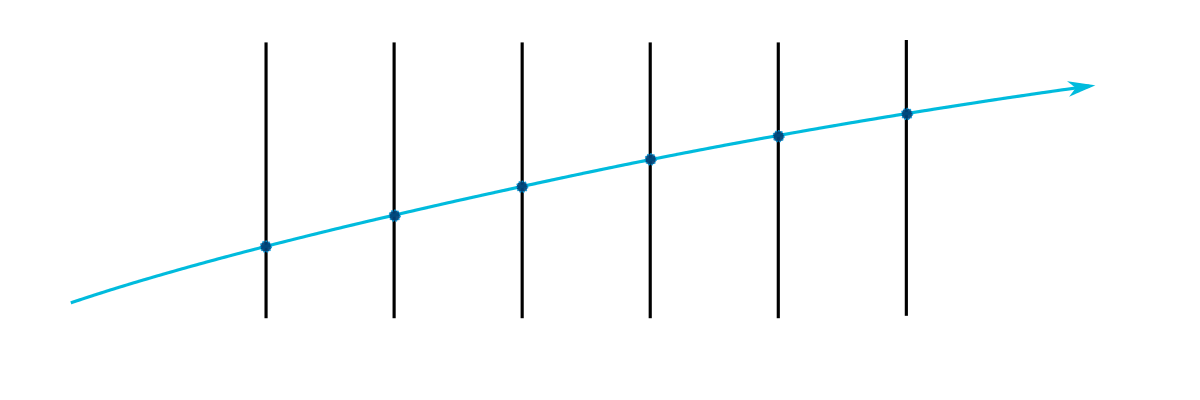
\includegraphics[width=0.45\textwidth]{../figs/Alignment/toyTracker03.png}
        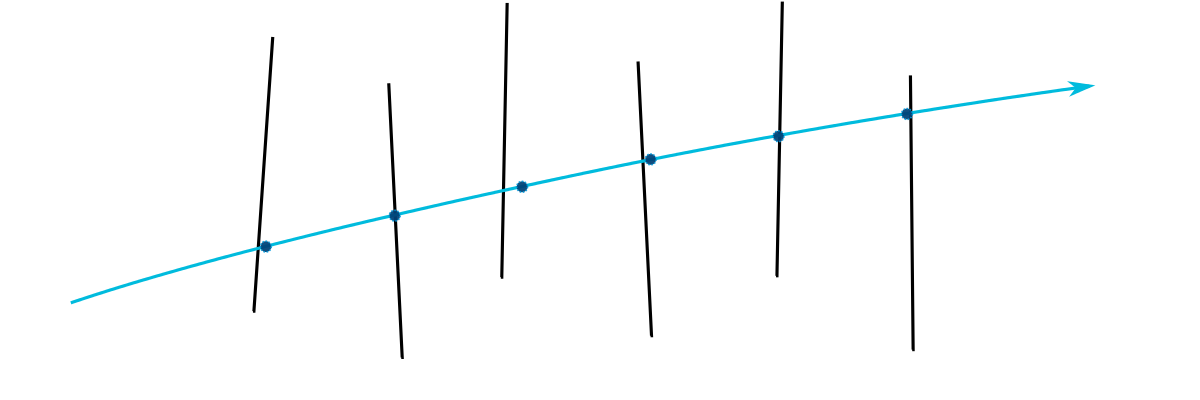
\includegraphics[width=0.45\textwidth]{../figs/Alignment/toyTracker04.png}
        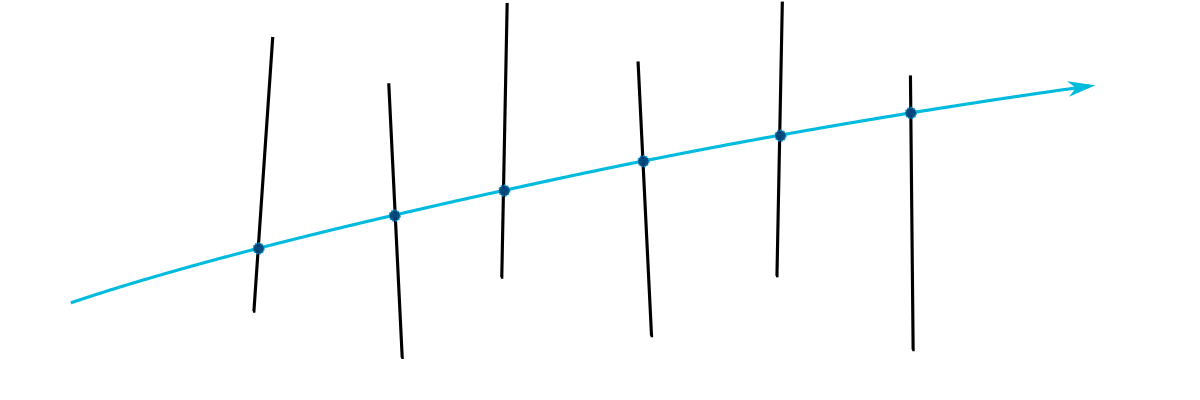
\includegraphics[width=0.45\textwidth]{../figs/Alignment/toyTracker05.png}
        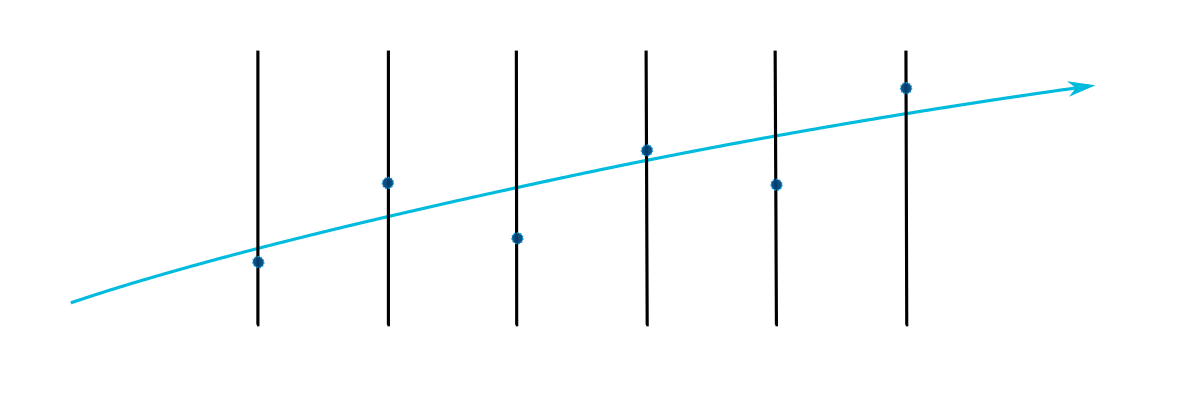
\includegraphics[width=0.45\textwidth]{../figs/Alignment/toyTracker06.png}
    \end{center}
    \caption{The alignment of a toy tracker, part 1.}
    \label{fig:toyTracker_part1}
\end{figure}

\begin{figure}[htb]
    \begin{center}
        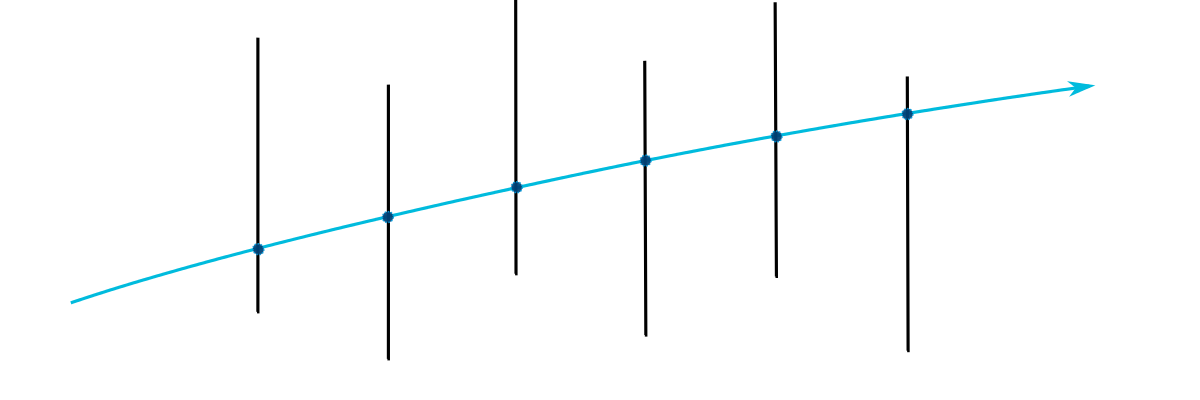
\includegraphics[width=0.45\textwidth]{../figs/Alignment/toyTracker07.png}
        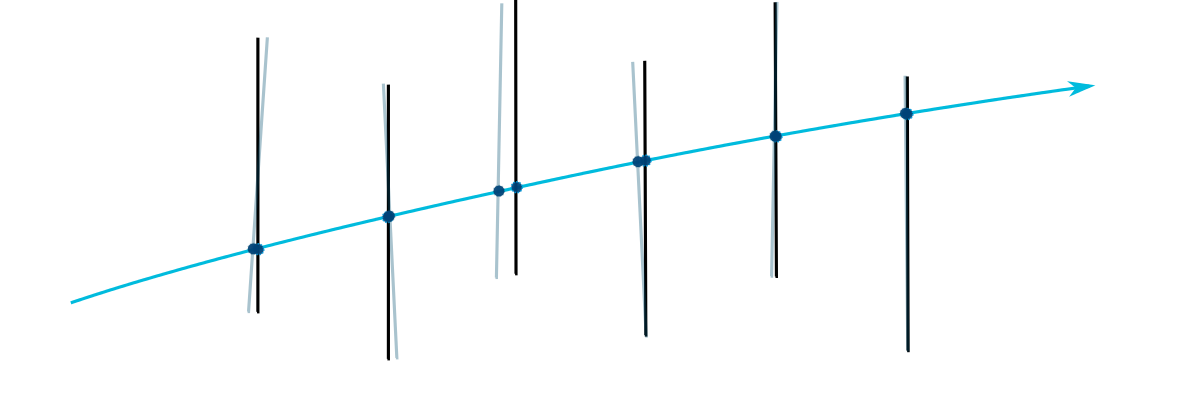
\includegraphics[width=0.45\textwidth]{../figs/Alignment/toyTracker08.png}
        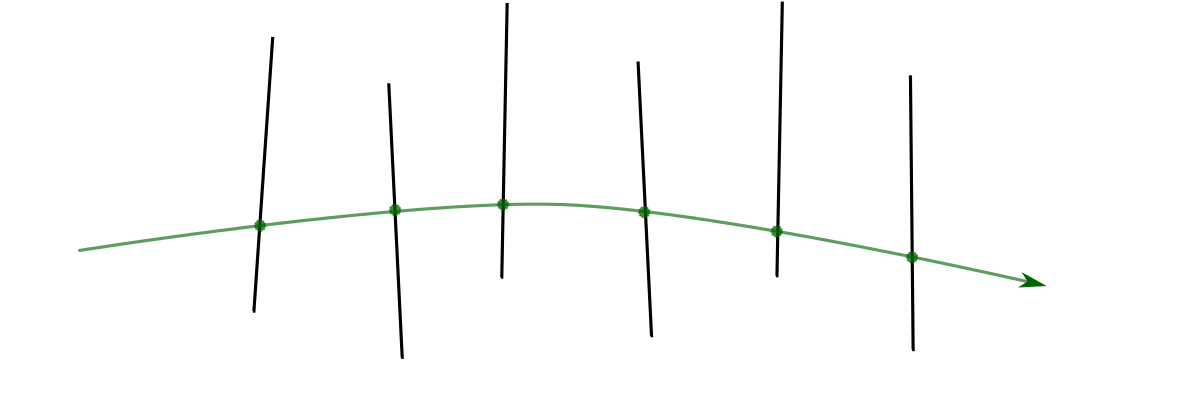
\includegraphics[width=0.45\textwidth]{../figs/Alignment/toyTracker09.png}
        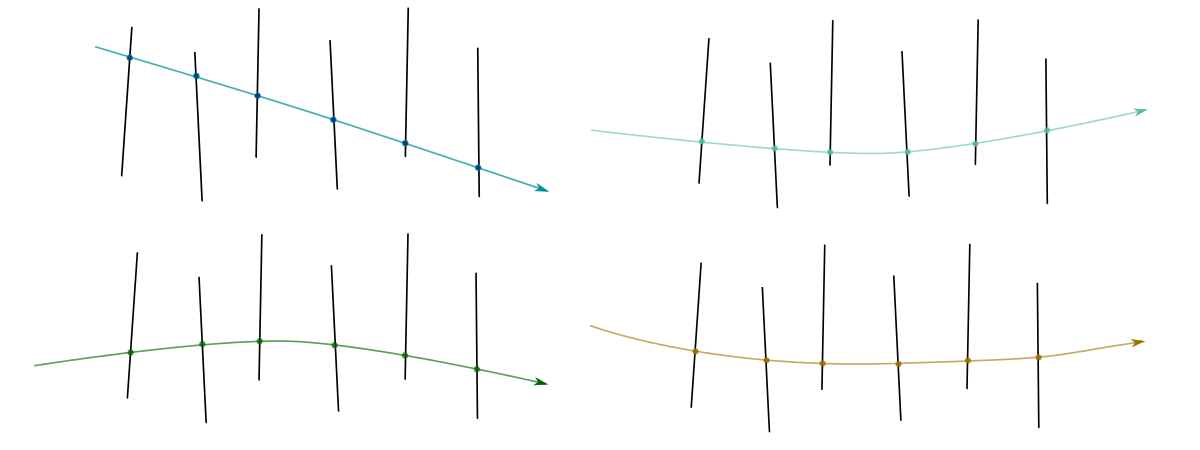
\includegraphics[width=0.45\textwidth]{../figs/Alignment/toyTracker10.png}
        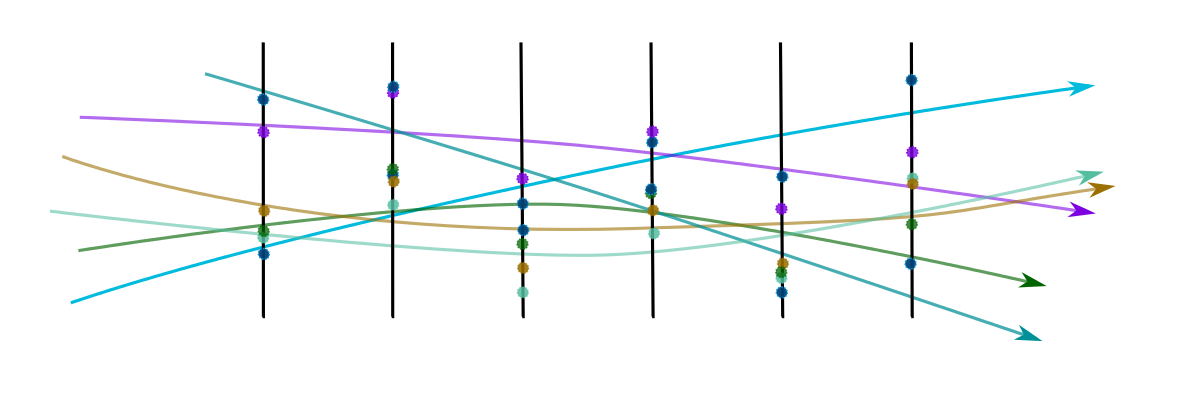
\includegraphics[width=0.45\textwidth]{../figs/Alignment/toyTracker12.png}
        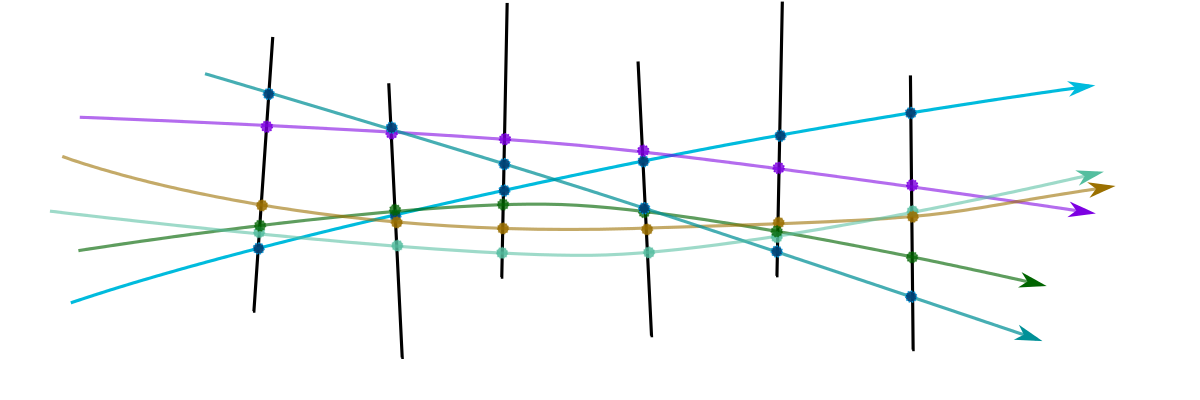
\includegraphics[width=0.45\textwidth]{../figs/Alignment/toyTracker13.png}
    \end{center}
    \caption{The alignment of a toy tracker, part 2.}
    \label{fig:toyTracker_part2}
\end{figure}

%The CMS tracker contains 1440 silicon pixel modules in PXB and PXF and 15148 silicon strip modules in TIB, TOB, TID, TEC. 

The tracker alignment problem is the least squared problem. The expression to minimize is the following:

\begin{equation}
  \chi^2(\mathbf{p},\mathbf{q})=\sum_j^{tracks} \sum_i^{hits} ({\frac{m_{ij}-f_{ij}(\mathbf{p},\mathbf{q_j})}{\sigma_{ij}}})^2
\end{equation}

where $\mathbf{p}$ are parameters describing the tracker geometry, $\mathbf{q}_j$ are parameters of the $j^{th}$ track, $m_{ij}-f_{ij}$ are residuals, distances between the measured hit and a position predicted by the track fit, $\sigma_{ij}$ is the Gaussian error of the measurement.

We have two alignment algorithms: Millepede and HIP. Milledepe performs a simoultaneous fit of all alignment parametes and all track parameters while HIP perform iterative fits of alignment parameters $\mathbf{p}$ and track parameters $\mathbf{q}_j$.

We can align the large substructures and individual modules with respect to their substructures. The parameters to align large substructures include their positions and orientations of the subdetectors (rotations). Thus, each subsystem is described by six parameters: three coordinates X, Y, Z and three angles $\alpha$, $\beta$, $\gamma$. At the module level, we align positions and rotations with respect to the positions and angles of the corresponding large structure (Fig.~\ref{fig:alignmentParameters}). In addition, at the module level we align for surface deformations which are described by three parameters per sensor (Fig.~\ref{fig:surfaceDeformations}). 

It is important to use different sorts of tracks for the alignment. Cosmic tracks pass through the detector vertically and do not allow us to connect different subdetectors to one another. Collision tracks originate from the collision point and go in all directions. However, those tracks which cross TEC are all almost collinear and, therefore, it is difficult to measure $z$-coordinate of TEC modules with collision tracks only.

\begin{figure}[htb]
    \begin{center}
        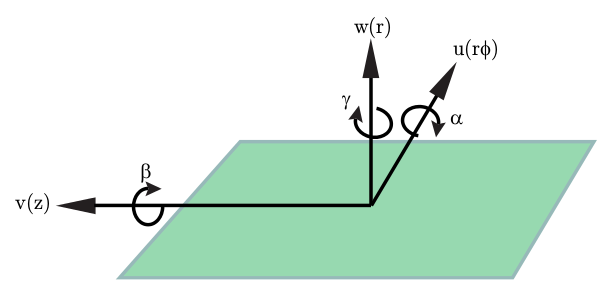
\includegraphics[width=0.70\textwidth]{../figs/Alignment/alignment_strip_coords.png}
    \end{center}
    \caption{Alignment parameters.}
    \label{fig:alignmentParameters}
\end{figure}

\begin{figure}[htb]
    \begin{center}
        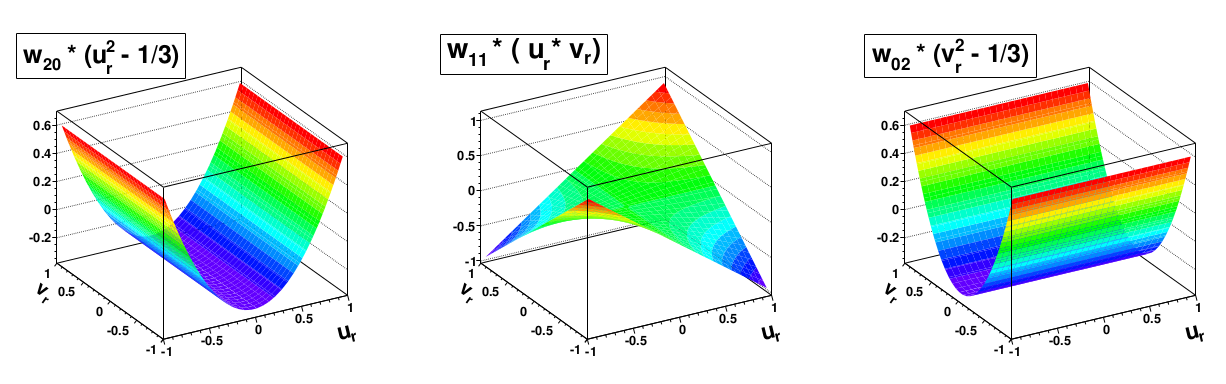
\includegraphics[width=0.90\textwidth]{../figs/Alignment/alignment_surface_deformations.png}
    \end{center}
    \caption{Surface deformations.}
    \label{fig:surfaceDeformations}
\end{figure}

It is necessary to align a part of the tracking system every time when we suspect a physical change in a location or an orientation this part. First of all, every time when CMS is taken out and placed back, all large structures need to be realigned. Also whenever a magnet is turned on and off, different parts of tracking system may shifts with respect to one another. Pixel half barrels are not screwed firmly, they are moving along each other on rails and, therefore, need to be realigned every~15 minutes. Realignment on the module level is necessary when modules are replaced. Also, module deformations may change when temperature changes. 

After the procedure of the tracking system alignment is performed, it is necessary to validate the results. Various tools of alignment validation are discussed in Chapter~\ref{sec:alignmentResults} using the example of the tracking system alignment based on the first Run~II data.   

%\begin{figure}[htb]
%    \begin{center}
%        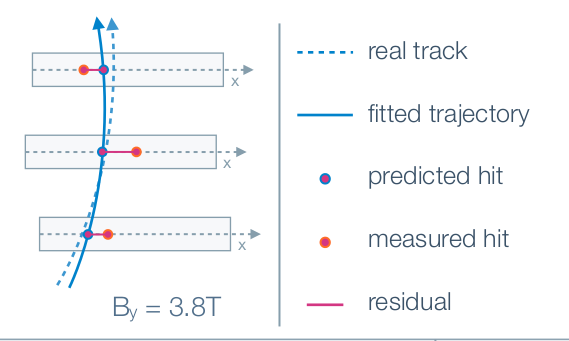
\includegraphics[width=0.70\textwidth]{../figs/Alignment/track.png}
%    \end{center}
%    \caption{Track residuals.}
%    \label{fig:trackAndResiduals}
%\end{figure}

%\begin{figure}[htb]
%  \begin{center}
%    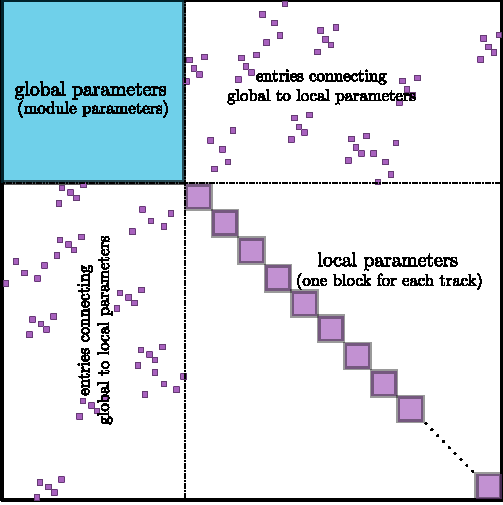
\includegraphics[width=0.70\textwidth]{../figs/Alignment/mpmatrix.pdf}
%  \end{center}
%  \caption{Track residuals.}
%  \label{fig:trackAndResiduals}
%\end{figure}
